
\documentclass[11pt,twocolumn, a4paper]{article}
\usepackage[utf8]{inputenc}
\usepackage{geometry}
\usepackage[pdftex]{graphicx}
\usepackage{setspace}
\usepackage{natbib}
\usepackage[scaled=0.9]{helvet}
\usepackage{colortbl}
\usepackage{color}
\usepackage{longtable}

\makeatletter
\def\s@btitle{\relax}
\def\subtitle#1{\gdef\s@btitle{#1}}
\def\@maketitle{%
  \newpage
  \null
  \vskip 2em%
  \begin{center}%
  \let \footnote \thanks
    {\LARGE \@title \par}%
                \if\s@btitle\relax
                \else\typeout{[subtitle]}%
                        \vskip .5pc
                        \begin{large}%
                                \textsl{\s@btitle}%
                                \par
                        \end{large}%
                \fi
    \vskip 1.5em%
    {\large
      \lineskip .5em%
      \begin{tabular}[t]{c}%
        \@author
      \end{tabular}\par}%
    \vskip 1em%
    {\large \@date}%
  \end{center}%
  \par
  \vskip 1.5em}
\makeatother 

\definecolor{gray}{rgb}{0.6,0.6,0.6}
\singlespacing
\paperwidth 8.5in
\paperheight 11in
\oddsidemargin 0in
\headsep 1.3cm 
\geometry{left=0.75in,top=0.75in,right=0.75in,bottom=0.75in}
\textwidth 7in 
\textheight 9.55in
\columnsep 0.4in
\footskip 0.4in 

\title{PL/JSON Reference Guide (version 0.8.1)}
\subtitle{For Oracle 10g and 11g}
\author{Jonas Krogsbøll}
\date{}

\begin{document}
\maketitle

\section*{PURPOSE}
The goal of PL/JSON is to create a correct implementation of JSON to use in a PL/SQL environments. The oracle object syntax is used because we want to be able to store JSON-objects in tables, without using character lobs. Parsing JSON-text and manual construction of JSON-objects should be easy as well as fetching data from the constructed objects should be. PL/JSON is delivered AS IS and we make no garantee for anything (although we think that the product is safe to use).

\section*{DESCRIPTION}
The parser and pretty-printer is implemented in two packages, but you'll never need to access these directly. The essential objects are linked to the relevant functions in the packages (in constructors and output methods). The two objects you should use are JSON and JSON\_LIST. You can consider the JSON object to be a mapping of strings to values and JSON\_LIST to be a list of values. The values that can be stored are the four primitives: JSON\_BOOL, JSON\_NULL, VARCHAR2 and NUMBER, plus JSON\_LIST and JSON as nested structures (see figure \ref{howjsonwork}).

\begin{figure}[!ht]
  \begin{center}
    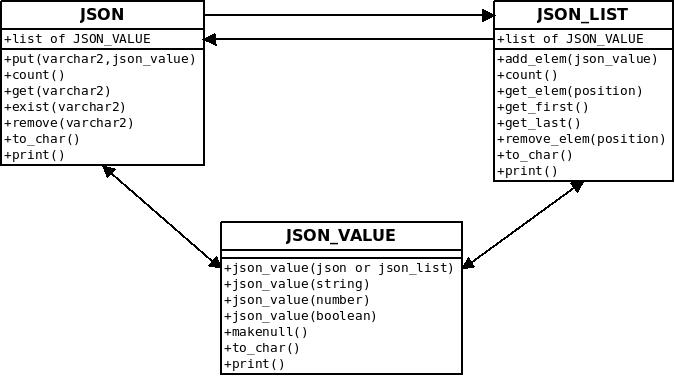
\includegraphics[width=0.8\linewidth]{visual.jpg}
  \end{center} 
  \caption{Essential Objects in PL/JSON}
  \label{howjsonwork}
\end{figure}

\section*{IN THE RELEASE}
\begin{itemize}
\item Install script
\item Uninstall script.
\item 8 new oracle types ready to use in your database.
\item 3 packages (parser, printer and extension)
\item A few examples files - does not modify the database.
\item Some testing script - creates and delete a table (JSON\_TESTSUITE)
\end{itemize}

\subsection*{Going from 0.6.2 to 0.8.0?}
Where did 0.7 go? Well, almost the entire code was rewritten. The API is very different now, so you cannot perform a simple upgrade from 0.6.2 to 0.8.0. Now there is no "to be implemented" methods. Additional methods (toClob, toRAW, etc.) will be added when they are ready and properly tested. The author of JSON thinks thats the way to go too: 
\begin{quotation}
We are finding that people like products that just work. It turns out that designs that just work are much harder to produce than designs that assemble long lists of features.\\ - Douglas Crockford (JavaScript: The Good Parts page 99)
\end{quotation}

\section*{KNOWN LIMITATIONS}
People hate limitations, but frustration kicks in when the limitations are unknown or undescribed. 
\begin{itemize}
\item The maximum input size the parser can accept is 32000 characters.
\item The pretty-printer limits it's output to 32676 characters (extra space added for line breaks and spaces).
\item Each string (pair-name or value) is limited to 4000 characters.
\item The number parsing assumes that oracles number type can contain the input (in most cases it can).
\end {itemize}

\subsection*{Example to workaround the pretty-printer size limit}
Suppose we want to build a large json-list and print it with dbms\_output.put\_line:
\small
\begin{verbatim}
declare
  obj json := json('{ 
    "test": true, 
    "array": [1,2,3]}');
  thelist json_list := json_list();
begin
  for i in 1 .. 300 loop
    obj.put('Loop counter', i);
    thelist.add_elem(obj.to_anydata);
  end loop;

  --printing starts
  dbms_output.put('[');
  for i in 1 .. thelist.count loop
    obj := json.to_json(thelist.get_elem(i));
    dbms_output.put(obj.to_char);
    if(i != thelist.count) then 
      dbms_output.put(', '); 
    end if;
  end loop;
  dbms_output.put_line(']');
end;
\end{verbatim}
\normalsize
Now the limitation will be the size of the dbms\_output buffer.

\section*{GETTING STARTED}
To get started on using this product, you should first install the product with the install script and then take a look at the examples in the \em examples \em folder. The content of each example file is:
\begin{itemize}
\item \textbf{ex1.sql}: Simple creation of a JSON object. 
\item \textbf{ex2.sql}: Simple creation of a JSON list. 
\item \textbf{ex3.sql}: Working with parser exceptions.
\item \textbf{ex4.sql}: Building an object with the API.
\item \textbf{ex5.sql}: Building a list with the API.
\item \textbf{ex6.sql}: Working with variables as copies.
\item \textbf{ex7.sql}: Using the extension package.
\item \textbf{sqlplus\_run.sql}: Displaying examples from www.json.org/example.html
\end{itemize}

\section*{EXTENSION PACKAGE}
The extension package makes it easier to work with the values in a JSON object or a JSON\_LIST. The values are all stored as ANYDATA, but can be converted back to a useful type with the static functions in the JSON object type. To know what conversion function you should use, you can test the value with the type testing functions in the JSON\_EXT package. The extension package also delivers a way of using dates in JSON, but you might ask why that functionality isn't a part of the object types. \\
The core implementation strictly follows the specification (RFC 4627 - http://www.ietf.org/rfc/rfc4627.txt?number=4627) on JSON. Furthermore the design goals with JSON were to, quote: ''be minimal, portable, textual and a subset of JavaScript. The less we need to agree on in order to interoperate, the more easily we can interoperate'' - D.Crockford. I, for instance, like dates/timestamp to be represented as milliseconds since 1st of January 1970 at 00:00:00 UTC. That is compact, but in a oracle context that isn't exactly the ideal choice. 

\section*{TESTSUITE}
Any proper product is tested for correctness. So should PL/JSON be with a testsuite that can be executed without installing any additional software on your database. You properly don't need the testsuite, but if you modify the implementation, adds more features, tests will be needed. Also if you discover a bug, you could report the bug by writing a relevant testcase.

\section*{CONTRIBUTING}
Write to us in the forums of sourceforge.net. We will be happy to hear from you. \\\\
Q: ''I've added a lot of code, please merge my changes''\\
A: Hmmm - it's not that we don't appriciate your work, but we would really prefer that you wrote tests and documentation to each feature - otherwise new code could easily break functionality. \\\\
Q: ''I've added some changes and I might contribute them to the project, but what's in it for me?''\\
A: This is not GPL, so you can keep your changes if you want to. 
When you are contributing then more eyes will look at your code. 
Possible errors might get detected and corrected and new features may arrise from your features - making it a better product you can use.

\section*{FUTURE PLANS}
Maybe an XPATH way of accessing and storing values will be implemented.\\
Additional json-list or json operations such at concat, substract, join, union, etc.\\
Enhancing the parser and printer to handle larger strings than 32K.\\
Test/example of storing json in a table.\\


\onecolumn
\section*{TYPES}
Example of usage can be found in the \em example \em folder. The important object types installed are JSON, JSON\_List, JSON\_BOOL and JSON\_NULL.

\begin{longtable}{| l | l |}
\hline
  \rowcolor{gray}\color{white}\textbf{TYPE NAME} & \color{white}\textbf{JSON} \\
\hline

\hline
  \textbf{CONSTRUCTOR} & json()\\
\hline
  \multicolumn{2}{|p{15cm}|}{Returns an empty JSON-object} \\
\hline

\hline
  \textbf{CONSTRUCTOR} & json(varchar2)\\
\hline
  \multicolumn{2}{|p{15cm}|}{Parses an json-text and return a JSON-object. 
Throws ORA-20101 and ORA-20100 in case of an faulty json-text.} \\
\hline

\hline
  \textbf{MEMBER PROCEDURE} & put(varchar2, anydata, position)\\
  & put(varchar2, varchar2, position)\\
  & put(varchar2, number, position)\\
  & put(varchar2, json\_bool, position)\\
  & put(varchar2, json\_null, position)\\
  & put(varchar2, json\_list, position)\\
  & put(varchar2, json, position)\\
\hline
  \multicolumn{2}{|p{15cm}|}{Adds a pair to the JSON-object. If the pair-name is allready present, then the value is replaced. If position is null (default) or larger than the number of pairs, the pair is inserted as a new last pair. If position < 2, the pair is inserted as a new first pair. Otherwise the pair is inserted at the specified position (list is 1-indexed). If the insertion value is null, a json\_null will be inserted (except for varchar2s).} \\
\hline

\hline
  \textbf{MEMBER FUNCTION} & count\\
\hline
  \multicolumn{2}{|p{15cm}|}{Returns the amount of pairs in the JSON-object (not counting nested object pairs).} \\
\hline

\hline
  \textbf{MEMBER FUNCTION} & get(varchar2)\\
\hline
  \multicolumn{2}{|p{15cm}|}{Returns the pair-value as ANYDATA if the pair exists (NULL otherwise). Convert ANYDATA to a useable object with the static functions.} \\
\hline

\hline
  \textbf{MEMBER FUNCTION} & exist(varchar2)\\
\hline
  \multicolumn{2}{|p{15cm}|}{Returns TRUE if the pair exists, FALSE otherwise} \\
\hline

\hline
  \textbf{MEMBER PROCEDURE} & remove(varchar2)\\
\hline
  \multicolumn{2}{|p{15cm}|}{Removes a pair from the JSON-object} \\
\hline

\hline
  \textbf{MEMBER FUNCTION} & to\_char\\
\hline
  \multicolumn{2}{|p{15cm}|}{Pretty-prints the JSON-object into a VARCHAR2} \\
\hline

\hline
  \textbf{MEMBER PROCEDURE} & print\\
\hline
  \multicolumn{2}{|p{15cm}|}{Outputs to\_char with dbms\_output.put\_line.} \\
\hline

\hline
  \textbf{MEMBER FUNCTION} & to\_anydata\\
\hline
  \multicolumn{2}{|p{15cm}|}{Convert the JSON-object into an ANYDATA value. Useful when inserting a JSON-object in a list.} \\
\hline

\hline
  \textbf{STATIC FUNCTION} & to\_json\\
\hline
  \multicolumn{2}{|p{15cm}|}{ANYDATA to JSON} \\
\hline
\hline
  \textbf{STATIC FUNCTION} & to\_json\_list\\
\hline
  \multicolumn{2}{|p{15cm}|}{ANYDATA to JSON\_LIST} \\
\hline
\hline
  \textbf{STATIC FUNCTION} & to\_json\_bool\\
\hline
  \multicolumn{2}{|p{15cm}|}{ANYDATA to JSON\_BOOL} \\
\hline
\hline
  \textbf{STATIC FUNCTION} & to\_json\_null\\
\hline
  \multicolumn{2}{|p{15cm}|}{ANYDATA to JSON\_NULL} \\
\hline
\hline
  \textbf{STATIC FUNCTION} & to\_number\\
\hline
  \multicolumn{2}{|p{15cm}|}{ANYDATA to NUMBER} \\
\hline
\hline
  \textbf{STATIC FUNCTION} & to\_varchar2\\
\hline
  \multicolumn{2}{|p{15cm}|}{ANYDATA to VARCHAR2} \\
\hline

\end{longtable}

\begin{longtable}{| l | l |}

\hline
  \rowcolor{gray}\color{white}
  \textbf{TYPE NAME} & \color{white}\textbf{JSON\_LIST} \\
\hline

\hline
  \textbf{CONSTRUCTOR} & json\_list()\\
\hline
  \multicolumn{2}{|p{15cm}|}{Returns an empty JSON\_LIST-object} \\
\hline

\hline
  \textbf{CONSTRUCTOR} & json\_list(varchar2)\\
\hline
  \multicolumn{2}{|p{15cm}|}{Parses an json-text and return a JSON\_LIST-object. 
Throws ORA-20101 and ORA-20100 in case of an faulty json-text.} \\
\hline

\hline
  \textbf{MEMBER PROCEDURE} & add\_elem(anydata, position)\\
& add\_elem(varchar2, position)\\
& add\_elem(number, position)\\
& add\_elem(json\_bool, position)\\
& add\_elem(json\_null, position)\\
& add\_elem(json\_list, position)\\
& add\_elem(json, position)\\
\hline
  \multicolumn{2}{|p{15cm}|}{Adds a value to the JSON\_LIST-object. If position is null (default) or larger than the length of the list, the value is inserted as a new last. If position < 2, the value is inserted as a new first. Otherwise the value is inserted at the specified position (note the the list is 1-indexed). If the insertion value is null, a json\_null will be inserted (except for varchar2s).} \\
\hline

\hline
  \textbf{MEMBER FUNCTION} & count\\
\hline
  \multicolumn{2}{|p{15cm}|}{Returns the amount of values in the JSON\_LIST-object (not counting nested list).} \\
\hline

\hline
  \textbf{MEMBER FUNCTION} & get\_elem(position)\\
\hline
  \multicolumn{2}{|p{15cm}|}{Returns the as ANYDATA if the value exists (NULL otherwise). Convert ANYDATA to a useable object with the JSON static functions.} \\
\hline

\hline
  \textbf{MEMBER FUNCTION} & get\_first\\
\hline
  \multicolumn{2}{|p{15cm}|}{ = list.get\_elem(1)} \\
\hline
\hline
  \textbf{MEMBER FUNCTION} & get\_last\\
\hline
  \multicolumn{2}{|p{15cm}|}{ = list.get\_elem(list.count)} \\
\hline

\hline
  \textbf{MEMBER FUNCTION} & remove\_elem(position)\\
\hline
  \multicolumn{2}{|p{15cm}|}{Remove the entry if it exists (assures that there are no \"holes\" in the list).} \\
\hline

\hline
  \textbf{MEMBER FUNCTION} & remove\_first\\
\hline
  \multicolumn{2}{|p{15cm}|}{ = list.remove\_elem(1)} \\
\hline
\hline
  \textbf{MEMBER FUNCTION} & remove\_last\\
\hline
  \multicolumn{2}{|p{15cm}|}{ = list.remove\_elem(list.count)} \\
\hline

\hline
  \textbf{MEMBER FUNCTION} & to\_char\\
\hline
  \multicolumn{2}{|p{15cm}|}{Pretty-prints the JSON\_LIST-object into a VARCHAR2} \\
\hline

\hline
  \textbf{MEMBER PROCEDURE} & print\\
\hline
  \multicolumn{2}{|p{15cm}|}{Outputs to\_char with dbms\_output.put\_line.} \\
\hline

\end{longtable}

\begin{longtable}{| l | l |}

\hline
  \rowcolor{gray}\color{white}
  \textbf{TYPE NAME} & \color{white}\textbf{JSON\_BOOL} \\
\hline

\hline
  \textbf{CONSTRUCTOR} & json\_bool(boolean)\\
\hline
  \multicolumn{2}{|p{15cm}|}{Returns an JSON\_BOOL-object (TRUE or FALSE)} \\
\hline

\hline
  \textbf{MEMBER FUNCTION} & to\_char \\
\hline
  \multicolumn{2}{|p{15cm}|}{'true' or 'false'} \\
\hline

\hline
  \textbf{MEMBER FUNCTION} & is\_true \\
\hline
  \multicolumn{2}{|p{15cm}|}{TRUE or FALSE} \\
\hline

\hline
  \textbf{MEMBER FUNCTION} & is\_false \\
\hline
  \multicolumn{2}{|p{15cm}|}{FALSE or TRUE} \\
\hline

\hline
  \textbf{STATIC FUNCTION} & maketrue \\
\hline
  \multicolumn{2}{|p{15cm}|}{json\_bool(TRUE)} \\
\hline

\hline
  \textbf{STATIC FUNCTION} & makefalse \\
\hline
  \multicolumn{2}{|p{15cm}|}{json\_bool(FALSE)} \\
\hline

\end{longtable}

\begin{longtable}{| l | l |}

\hline
  \rowcolor{gray}\color{white}
  \textbf{TYPE NAME} & \color{white}\textbf{JSON\_NULL} \\
\hline

\hline
  \textbf{CONSTRUCTOR} & json\_bool(boolean)\\
\hline
  \multicolumn{2}{|p{15cm}|}{Returns an JSON\_BOOL-object (TRUE or FALSE)} \\
\hline

\hline
  \textbf{MEMBER FUNCTION} & to\_char \\
\hline
  \multicolumn{2}{|p{15cm}|}{'true' or 'false'} \\
\hline

\hline
  \textbf{MEMBER FUNCTION} & is\_true \\
\hline
  \multicolumn{2}{|p{15cm}|}{TRUE or FALSE} \\
\hline

\hline
  \textbf{MEMBER FUNCTION} & is\_false \\
\hline
  \multicolumn{2}{|p{15cm}|}{FALSE or TRUE} \\
\hline

\hline
  \textbf{STATIC FUNCTION} & maketrue \\
\hline
  \multicolumn{2}{|p{15cm}|}{json\_bool(TRUE)} \\
\hline

\hline
  \textbf{STATIC FUNCTION} & makefalse \\
\hline
  \multicolumn{2}{|p{15cm}|}{json\_bool(FALSE)} \\
\hline

\end{longtable}

\section*{Test environments}
Tested on Oracle Database 10g Express Edition 10.2.0.1.0 @ Ubuntu 9.04 (x86)\\
Tested on Oracle Database 10gR2 Enterprise Edition 10.2.0.2.0 @ Windows Server 2003 (x64)

\end{document}



